\documentclass{article}

\usepackage{graphicx}
\usepackage{tikz}
\usepackage{tikzsymbols}
\usetikzlibrary{calc,patterns,shapes.geometric}
\pagestyle{empty}
\usepackage[margin=0pt]{geometry}
\geometry{papersize={14in,12in}}

\def\centerarc[#1](#2)(#3:#4:#5){\draw[#1] ($(#2)+({#5*cos(#3)},{#5*sin(#3)})$) arc (#3:#4:#5);}

\begin{document}
	\begin{figure}
		\centering
		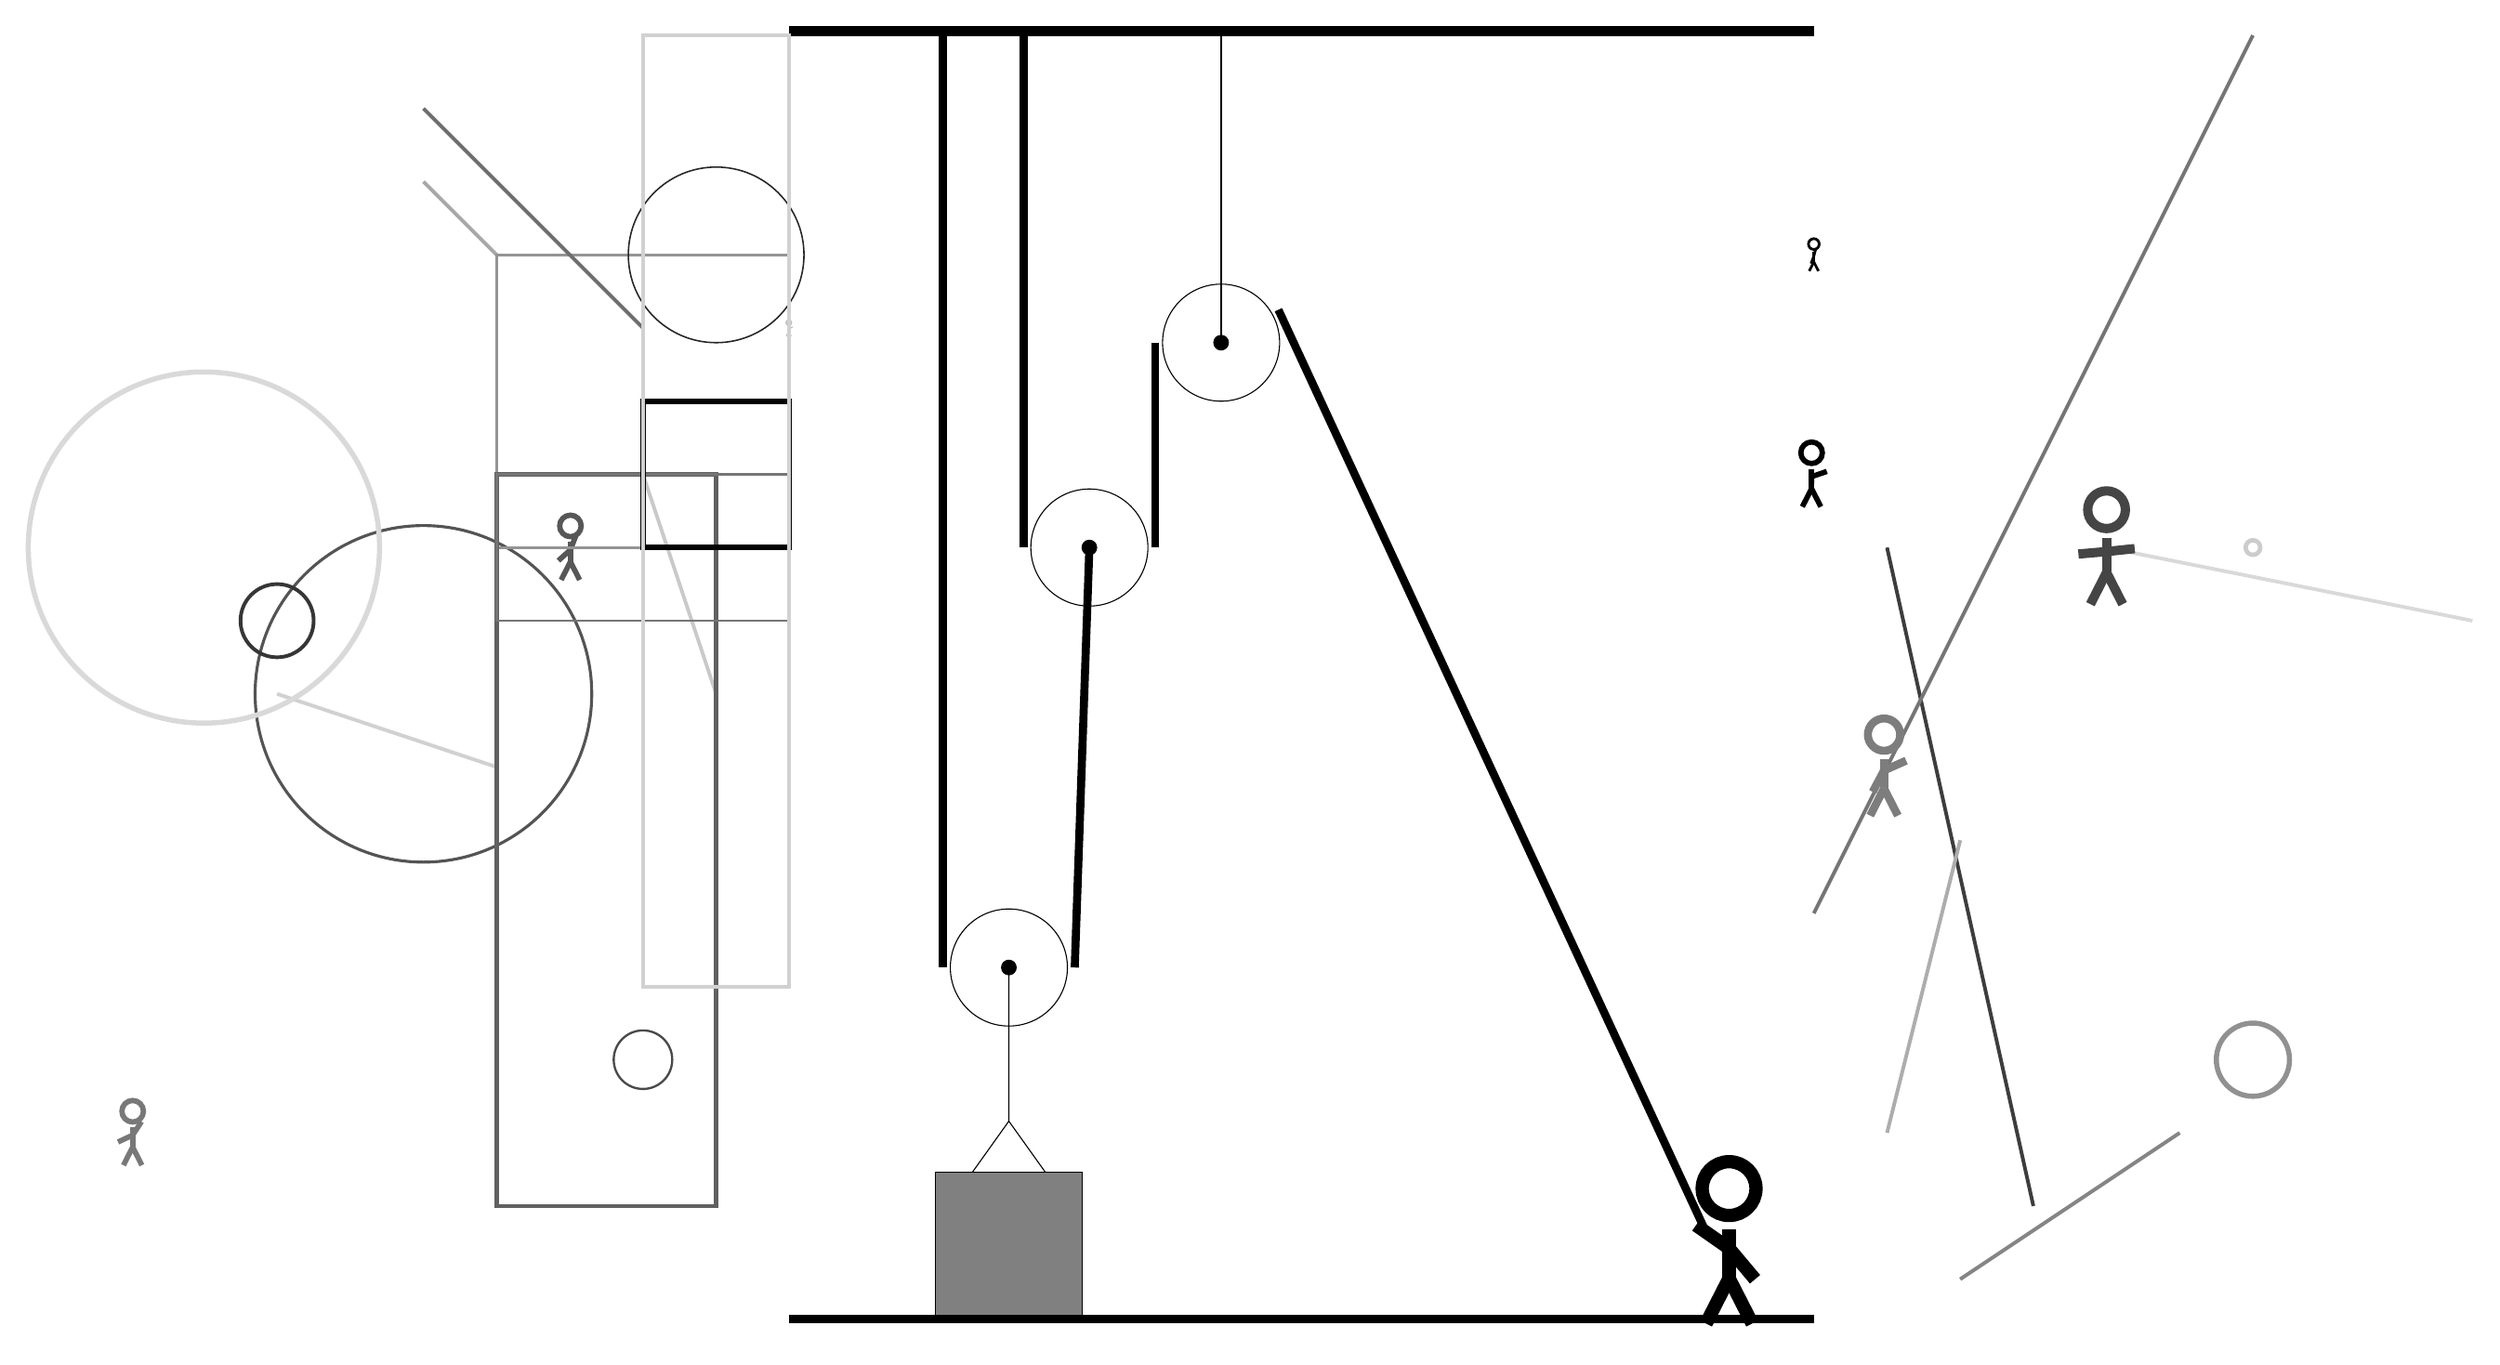
\begin{tikzpicture}
			%%%%% START %%%%%
			
			\draw[fill=black] (-2, 14) rectangle (12, 14.125);
			
			\draw (1, 1.26) circle (0.8);
			\draw[fill=black] (1, 1.26) circle (0.1);
			
			\draw (2.1, 7.0) circle (0.8);
			\draw[fill=black] (2.1, 7.0) circle (0.1);
			
			\draw[line width=0.5mm, color=black!18](-6, 4) -- (-9, 5);
			
			\draw[line width=0.5mm, color=black!34](-6, 11) -- (-7, 12);
			\node[line width=0.7mm, color=black!97] at (12, 11) {\Strichmaxerl[2][70][75]};
			\draw [line width=0.4mm, color=black!67](-7, 5) circle (2.3);
			\node[line width=0.3mm, color=black!100] at (12, 8) {\Strichmaxerl[4][89][19]};
			\draw[line width=0.5mm, color=black!76](13, 7) -- (15, -2);
			
			\node[line width=0.7mm, color=black!66] at (-5, 7) {\Strichmaxerl[4][42][69]};
			\draw[line width=0.4mm, color=black!42] (-2, 11) rectangle (-6, 7);
			\draw[line width=0.5mm, color=black!62] (-2, 8) rectangle (-4, 9);
			\draw [line width=0.2mm, color=black!85](-3, 11) circle (1.2);
			\node[line width=0.7mm, color=black!26] at (-2, 10) {\Strichmaxerl[1][83][22]};
			\draw [line width=0.6mm, color=black!20](18, 7) circle (0.1);
			\draw[line width=0.5mm, color=black!21](-4, 8) -- (-3, 5);
			
			\draw [line width=0.5mm, color=black!79](-9, 6) circle (0.5);
			\draw [line width=0.7mm, color=black!43](18, 0) circle (0.5);
			\draw[line width=0.6mm, color=black!62] (-3, -2) rectangle (-6, 8);
			
			\draw[line width=0.5mm, color=black!32](14, 3) -- (13, -1);
			\node[line width=0.2mm, color=black!53] at (-11, -1) {\Strichmaxerl[4][25][57]};
			\draw [line width=0.7mm, color=black!15](-10, 7) circle (2.4);
			\draw[line width=0.5mm, color=black!54](12, 2) -- (18, 14);
			\draw[line width=0.5mm, color=black!15](16, 7) -- (21, 6);
			
			\draw[line width=0.3mm, color=black!54] (-2, 8) rectangle (-6, 6);
			\draw[line width=0.5mm, color=black!48](17, -1) -- (14, -3);
			\node[line width=0.3mm, color=black!51] at (13, 4) {\Strichmaxerl[6][62][24]};
			\node[line width=0.7mm, color=black!73] at (16, 7) {\Strichmaxerl[7][5][6]};
			
			\draw[line width=0.7mm, color=black!99] (-2, 7) rectangle (-4, 9);
			\draw[line width=0.5mm, color=black!57](-4, 10) -- (-7, 13);
			\draw [line width=0.3mm, color=black!71](-4, 0) circle (0.4);
			
			\draw[line width=0.5mm, color=black!18] (-4, 14) rectangle (-2, 1);
			
			\draw (3.9, 9.8) circle (0.8);
			\draw[fill=black] (3.9, 9.8) circle (0.1);
			\draw[thick] (3.9, 9.8) -- (3.9, 14);
			
			\draw (1, 1.26) -- (1, -0.84) -- (0.5, -1.54) -- (1.5, -1.54) -- (1, -0.84);
			\draw[fill=black!50] (0, -1.54) rectangle (2, -3.54);
			
			\draw[line width=1.1mm] (0.1, 14) -- (0.1, 1.26);
			\centerarc[line width=1.1mm](1, 1.26)(180:360:0.9);
			\draw[line width=1.1mm](1.9, 1.26) -- (2.1, 7.0);
			\draw[line width=1.1mm] (1.2, 14) -- (1.2, 7.0);
			\centerarc[line width=1.1mm](2.1, 7.0)(180:360:0.9);
			\draw[line width=1.1mm](3.0, 7.0) -- (3.0, 9.8);
			\centerarc[line width=1.1mm](3.9, 9.8)(30:180:0.9);
			\draw[line width=1.1mm] (4.683, 10.25) -- (10.5, -2.3);
			
			\node at (10.8, -2.5) {\Strichmaxerl[10][-35][-50]};
			
			\draw[fill=black] (-2, -3.5) rectangle (12, -3.6);
			
			%%%%% END %%%%%
		\end{tikzpicture}
	\end{figure}	
\end{document}